\section{结果}
\label{sec:results}
\subsection{契约与操作边界}
全部 22 项选定反例测试逐项在与上下文诊断相同的保留可执行文件上重放，均通过。每次调用报告一项通过、零项失败和零项忽略，均未超时。每次调用前后的可执行文件哈希一致，774 路径源码清单、全部 1003 个归档源码文件以及主原始报告均未发生变化。表~\ref{tab:counterexamples} 对所测试的边界进行分组。

\begin{table}[t]
\small
\caption{在保留可执行文件上重放的选定反例。每项测试执行一次。计数表示预期行为成功出现的次数，不是通过抽样得到的失败检出准确率。}
\label{tab:counterexamples}
\begin{tabularx}{\columnwidth}{@{}Xr@{}}
\toprule
边界与所测试的区别 & 通过数\\
\midrule
验收：修订、回执、权威性与批准条件 & 11/11\\
生产者冲突：另一生产者通过后，适用失败仍保留 & 2/2\\
依赖归属：不确定的映射仍附有限定 & 2/2\\
范围与可观测性：未解决工作与验证状态 & 2/2\\
评价器：构造反例下的评分行为 & 5/5\\
\midrule
总计 & 22/22\\
\bottomrule
\end{tabularx}
\end{table}

这些测试给出了第~\ref{sec:contract} 节契约的具体实例：修订或权威性不匹配的结果不能提供必需的支持证据；另一生产者的通过记录也不能移除适用的阻断失败。测试结果在所用夹具下验证了选定断言，并不证明任意验证计划都充分，也不证明能够抵御自适应攻击。这些测试的先前执行使用另一构建；本次重放消除了这一来源差异，但未将两次执行合并。

十一项主控制检查全部通过。在竞争写入检查中，两次操作以相同的已观察哈希开始；一次提交成功，另一次被拒绝。只读与工作区边界控制检查拒绝不符合条件的操作。不完整图报告保留其覆盖不完整状态。在语法缓存压力下，本次运行记录了 13,168 次裁减，仍报告 96 个文件、96 个匹配、零失败和完整覆盖。工作区相对路径下的验证请求合并通过了针对重复执行的检查。

这些控制检查在各自声明的粒度上支持 RQ1。例如，并发写入结果为所测试调度下受保护的单文件路径提供证据；它并不证明多文件编辑具备事务性，也不证明能够与所有外部进程正确协调。

\subsection{有界源码交付}
在每一种预算与缓存阶段组合下，身份、完整原始函数体交付以及当前文件元数据 SHA 均满足全部 686 项标注要求。所有 406 次符合编辑条件的尝试均满足严格的编辑输入谓词。六种条件合计对应 4116 个必需源码实例和 2436 次符合条件的编辑尝试。查询错误、响应超预算和预热错误均为零。

这些饱和结果回答了保留语料范围内的 RQ2，也揭示了该语料区分能力的局限：它所需的源码很小，即使最低预算也能容纳。因此，100\% 的源码分数几乎无法说明增加预算如何改变其他有用证据。图~\ref{fig:budget} 将饱和的交付指标与决策记录暴露率、实际响应大小并列，展示这种区别。

\begin{figure*}[t]
\centering
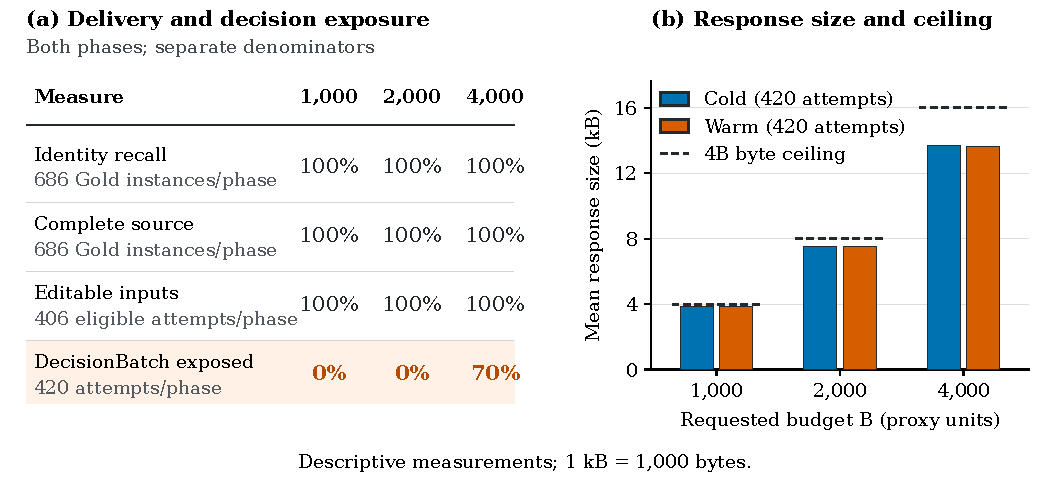
\includegraphics[width=\textwidth]{figures/budget_exposure.pdf}
\caption{预算对不同输出的影响并不相同。左：源码交付、编辑输入成功率和序列化决策记录暴露率采用不同分母（每种条件分别为 686 项源码要求、406 次符合条件的编辑尝试和 420 次总尝试）。冷态与预热态的各项比例一致；两个阶段的数据未合并。右：平均序列化响应字节数均低于计量规则对应的 $4B$ 上限。最低预算已经使源码交付指标达到饱和。}
\label{fig:budget}
\end{figure*}

\subsection{嵌套就绪谓词}
对于 RQ3，按尝试统计的身份、函数体以及函数体加文件元数据谓词，在每种条件下都将 413 次可回答观察判为阳性；完整的编辑输入谓词则判定 406 次为阳性。因此，省略写入资格条件会纳入七次只读观察，占可回答观察的 $7/413=1.69\%$。六种条件下受到影响的 42 次观察，都是同一个只读夹具的重复，不是独立发现的 42 个漏洞。

这一结果规模不大，但具有诊断意义。正确的定位、原始源码和新鲜哈希可能同时存在，编辑却仍不满足准入条件。移除额外的文件元数据 SHA 谓词，在本语料中没有带来进一步区分，因为前一层函数体谓词已经检查了源码窗口哈希。因此，该分析没有识别每个嵌套条件各自独立的因果效应，但确立了一个具体反例：源码可用不等于编辑就绪。

\subsection{预算、可见性与延迟}
在两个缓存阶段中，序列化 \code{DecisionBatch} 的暴露次数在预算 1000 和 2000 下均为 0/420，在预算 4000 下均为 294/420（70\%）。因此，相同的源码召回率并不意味着运行时结构化决策具有相同的可见性。这一发现回答了 RQ4 中关于可见性的部分，但没有将暴露的记录解释为真实任务上的正确决策。

\begin{table*}[t]
\centering\small
\caption{冻结主运行的描述性开销。每行包含 420 次实测调用。延迟分位数按调用汇总；图~\ref{fig:latency} 的经验累积分布函数（ECDF）则使用场景中位数。字节数指序列化 JSON 字节数，不是模型 token 数。}
\label{tab:cost}
\begin{tabular}{@{}rrcrrrr@{}}
\toprule
预算 $B$ & 字节上限 $4B$ & 阶段 & 平均字节数 & p50 (ms) & p95 (ms) & 决策暴露次数\\
\midrule
1000 & 4000 & 冷态 & 3850.14 & 40.186 & 70.913 & 0/420\\
1000 & 4000 & 预热态 & 3849.71 & 27.030 & 51.216 & 0/420\\
2000 & 8000 & 冷态 & 7506.04 & 34.795 & 61.286 & 0/420\\
2000 & 8000 & 预热态 & 7503.97 & 20.738 & 34.736 & 0/420\\
4000 & 16000 & 冷态 & 13667.22 & 25.709 & 56.378 & 294/420\\
4000 & 16000 & 预热态 & 13663.93 & 12.948 & 25.150 & 294/420\\
\bottomrule
\end{tabular}
\end{table*}

\begin{figure}[t]
\centering
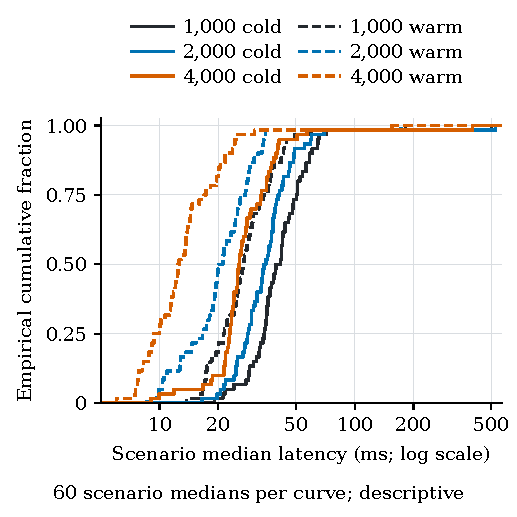
\includegraphics[width=\columnwidth]{figures/latency_ecdf.pdf}
\caption{场景中位数的延迟分布，延迟轴采用对数刻度。六条曲线各包含 60 个中位数，每个中位数来自七次重复调用。颜色表示预算，线型表示执行框架缓存阶段。全部观测中位数均予保留，包括分布的上尾。}
\label{fig:latency}
\end{figure}

在六种条件下，调用延迟中位数介于 12.948 和 40.186\,ms 之间，最大的 p95 为 70.913\,ms。预热态的汇总延迟均低于对应冷态。预算较大的条件在本次运行中也测得更低延迟，但这一关系尚不能证明预算增大带来了加速：固定的预算顺序、打包工作量、共享操作系统缓存和未受控制的主机负载都可能构成混杂因素。能够支持的结论是：在所声明的 debug 构建协议下，该主机上的调用中位数和第 95 百分位数处于数十毫秒量级；单次观察值及部分场景中位数仍延伸至更长的尾部。

综合结果揭示了三种彼此不同的状态：源码要求可以全部得到满足，编辑仍可能不符合准入条件，结构化决策记录也仍可能缺失。将其中任一指标当成通用的就绪分数，都会掩盖返回接口中可观察到的差异。
